\documentclass{article}

\usepackage[utf8]{inputenc}
%\usepackage{a4wide}
\usepackage{amsthm}
\usepackage{amsmath}
\usepackage{url}
\usepackage{algorithm}
\usepackage{algorithmic}
\usepackage{float}
\usepackage{tikz}
\usetikzlibrary{topaths,calc}

\title{Modèles graphiques probabilistes}
\author{Charles-Pierre Astolfi, Émile Contal} 
\date{3 janvier 2012}

\begin{document}
\newtheorem*{mdef}{Définition}
\newtheorem*{mthm}{Théorème}

\maketitle

\begin{abstract}
Le but de notre travail est d'évaluer un algorithme qui permet
d'approximer la largeur arborescente (treewidth) d'un graphe.

Beaucoup de problèmes de graphes (par exemple, l'inférence bayesienne)
peuvent être résolus en temps polynomial sur des graphes de largeur
arborescente bornée. Le calcul exact de la largeur arborescente est un
problème NP-complet et nécessite l'utilisation d'heuristiques. Ce
rapport est dédié à l'étude d'un de ces algorithmes, décrit dans
\cite{rootpaper}.

\end{abstract}

\section{Introduction}
Dans le cadre de l'article ``A Practical Relaxation of Constant-Factor
Treewidth Approximation Algorithms'' \cite{rootpaper}, nous avons
implémenté l'algorithme proposé et l'avons comparé à d'autres
algorithmes de calcul de treewidth.


\section{Théorie}

Nous commençons cette section par quelques définitions qui nous seront
utiles dans la suite.

\begin{mdef}
Soit $G = (V,E)$ un graphe non-orienté sans boucle. On dit que $G$ est
connecté s'il existe un chemin entre chaque paire de sommets de $G$.
\end{mdef}

\begin{mdef}
On dit que $G$ est triangulé si pour tout cycle de longueur supérieure
strictement à 3, il existe une arête entre deux sommets non-adjacents
du cycle. La largeur d'un graphe triangulé est la taille de sa plus
grande clique moins 1.
\end{mdef}

\begin{mdef}
La largeur arborescente d'un graphe est la largeur minimale obtenable
parmi toutes les triangulations possibles.
\end{mdef}

\begin{mdef}
Un \emph{dtree} d'un graphe $G$ non-orienté est un arbre binaire
complet, dont les feuilles sont les arêtes de $G$.
\end{mdef}
Il permet de guider les algorithmes de partitionnement de type
\emph{divide-et-conquere}.

\begin{mdef}
Le \emph{contexte} d'un noeud $t$ d'un dtree est l'ensemble des noeuds
qui représente le bord du sous-graphe $G(t)$ par rapport au graphe
$G$. C'est-à-dire qu'un noeud $v$ apparait dans le contexte de $t$ si
et seulement s'il y a $v-u$ dans $G$ avec $v$ dans $G(t)$ et $u$ hors
de $G(t)$.
\end{mdef}

\begin{mdef}
Le \emph{cutset} d'un noeud $t$ d'un dtree est l'ensemble des noeuds
communs à $G(t_l)$ et à $G(t_r)$ et qui ne sont pas dans le contexte
de $t$.
\end{mdef}

Il est facile de vérifier que $context(t)$ et $cutset(t)$ sont des
ensembles disjoints, ce qui motive la définition suivante : 

\begin{mdef}
$$
cluster(t) = \left\{
    \begin{array}{ll}
        vars(t) & \mbox{ si $t$ est une feuille} \\
        cutset(t) \cup context(t) & \mbox{ sinon.}
    \end{array}
\right.
$$
\end{mdef}

Ceci permet de définir la largeur d'un $dtree$ : 
\begin{mdef}
La \emph{largeur} d'un dtree est la taille de son plus gros cluster
moins 1.
\end{mdef}

Hopkins et Derwiche \cite{hop} ont proposé une transformation
polynomiale qui conserve la largeur entre un dtree et une
triangulation d'un graphe.
Un dtree de largeur $w$ d'un graphe $G$ permet
de construire une triangulation de même largeur
et ainsi borner la largeur arborescente de $G$ par $w$.

C'est cette remarque que nous exploitons dans les algorithmes
\ref{algo1} et \ref{algo2} pour calculer la treewidth.

Notre objectif est de donc construire un dtree de largeur la plus
petite possible ; pour ce faire on partitionne un hypergraphe $H(G)$
définit ainsi :
$$ H(G) = (E,\{ \{ (u,v) \in E \} \mid u \in V \}) $$
Chaque noeud du dtree est construit par partitionnement récursif de $H(G)$.

\paragraph{}
Robertson et Seymour \cite{robert} ont montré qu'il existe toujours
un partitionnement de $G(t)$ tel que chaque sous-graphe $G(t_l)$ et
$G(t_r)$ contient au moins $2/3$ des noeuds du contexte de $t$.  Un
tel partitionnement permet d'assurer que notre algorithme donnera une
approximation de la largeur arborescente d'au plus $4k+1$, avec $k$ la
largeur arborescente du graphe original. 

En pratique, nous n'avons aucune garantie de trouver un tel partitionnement,
cependant l'article affirme obtenir de très bons résultats.

\paragraph{}
Un exemple de graphe, d'hypergraphe correspondant et de dtree se
trouve dans les figures \ref{lol1}, \ref{lol2} et \ref{lol3}.
\newpage

\begin{figure}[H]
 \centering
\begin{tikzpicture}[auto, node distance=2cm]
  \node[] (1) {A};
  \node[below left of=1] (2) {B};
  \node[below right of=1] (3) {C};
  \node[below right of=2] (4) {D};
  \node[below right of=3] (5) {E};
 \path
  (1) edge node {} (2)
  (1) edge node {} (3)
  (2) edge node {} (3)
  (2) edge node {} (4)
  (3) edge node {} (4)
  (3) edge node {} (5);
\end{tikzpicture}
\caption{Exemple de graphe $G$}
\label{lol1}
\end{figure}

\begin{figure}[H]
\label{lol2}
  \centering
  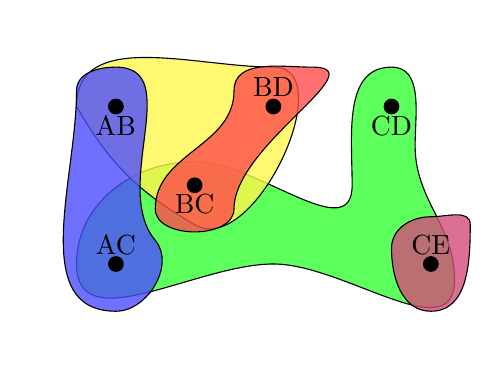
\begin{tikzpicture}
    \node (ab) at (0,2) {};
    \node (ac) at (0,0) {};
    \node (bc) at (1,1) {};
    \node (bd) at (2,2) {};
    \node (cd) at (3.5,2) {};
    \node (ce) at (4,0) {};

    \begin{scope}[fill opacity=0.8]
    \filldraw[fill=green!80] ($(ac)+(-0.5,0)$)
        to[out=90,in=180] ($(bc)+(0,0.3)$)
        to[out=0,in=270] ($(cd)+(-0.5,-1)$)
        to[out=90,in=180] ($(cd)+(0,0.5)$)
        to[out=0,in=90] ($(cd)+(0.3,-0.5)$)
        to[out=270,in=90] ($(ce)+(0.3,-0.2)$)
        to[out=270,in=0] ($(ce)+(-2,0)$)
        to[out=180,in=270] ($(ac)+(-0.5,0)$);
    \filldraw[fill=yellow!70] ($(ab)+(-0.5,0)$) 
        to[out=90,in=180] ($(bd) + (0,0.5)$) 
        to[out=0,in=330] ($(bc) + (0,-0.5)$)
        to[out=150,in=300] ($(ab)+(-0.5,0)$);
    \filldraw[fill=blue!70] ($(ab)+(-0.5,0.2)$)
        to[out=90,in=180] ($(ab)+(0,0.5)$)
        to[out=0,in=130] ($(ac)+(0.5,0.3)$)
        to[out=310,in=0] ($(ac)+(0,-0.6)$)
        to[out=180,in=270] ($(ab)+(-0.5,0.2)$);
    \filldraw[fill=red!70] ($(bd)+(-0.5,0.2)$)
        to[out=90,in=180] ($(bd)+(0.5,0.5)$)
        to[out=0,in=90] ($(bc)+(0.5,-0.3)$)
        to[out=270,in=270] ($(bc)+(-0.5,-0.3)$)
        to[out=90,in=270] ($(bd)+(-0.5,0.2)$);
     \filldraw[fill=purple!70] ($(ce)+(-0.5,0.2)$)
        to[out=90,in=180] ($(ce)+(0,0.6)$)
        to[out=0,in=90] ($(ce)+(0.5,0.5)$)
        to[out=270,in=0] ($(ce)+(0,-0.6)$)
        to[out=180,in=270] ($(ce)+(-0.5,0.2)$);
    \end{scope}

    \fill (ab) circle (0.1) node [below] {AB};
    \fill (ac) circle (0.1) node [above] {AC};
    \fill (bc) circle (0.1) node [below] {BC};
    \fill (bd) circle (0.1) node [above] {BD};
    \fill (cd) circle (0.1) node [below] {CD};
    \fill (ce) circle (0.1) node [above] {CE};
  \end{tikzpicture}
  \caption{Hypergraphe $H(G)$}
\end{figure}

\begin{figure}[H]
  \tikzstyle{internal} = [rectangle, draw]
  \tikzstyle{level 1} = [sibling distance=4cm]
  \tikzstyle{level 2} = [sibling distance=3cm]
  \tikzstyle{level 3} = [sibling distance=2cm]
  \tikzstyle{level 4} = [sibling distance=1.5cm]
  \centering
 \begin{tikzpicture}
    \node [internal] (0) {(\{B,C\}, \{\})}
    child{
      node [internal] (1) { (\{A\}, \{B,C\}) }
      child{
        node[] (2) { AB }
      }
      child{
        node[] (3) { AC }
      }
    }
    child{ 
      node [internal] (4) { (\{\}, \{B,C\}) }
      child{
        node[] (5) { CE }
      }
      child{
        node [internal] (6) { (\{\}, \{B,C\}) }
        child{
          node [] (7) {BC}
        }
        child {
          node [internal] (8)  { (\{D\}, \{B,C\}) }
          child{
            node[] (9) {CD}
          }
          child{
            node[] (10) {BD}
          }
        }
      }
    };
 \end{tikzpicture}
 \caption{Exemple de dtree de largeur $2=3-1$ du graphe $G$ avec les contextes et cutsets}
\label{lol3}
\end{figure}

\newpage

\section{Implémentation}
Nous avons réalisé l'implémentation en OCaml \cite{ocaml}, et le code
est disponible à l'adresse
\url{http://www.dptinfo.ens-cachan.fr/~cpastolf/treewidth.zip}

Le partitionnement de $H(G)$ est fait, comme dans l'article, grâce à
la librairie hMetis, qui utilise des heuristiques randomisées.
Pour chaque execution du programme, de nombreuses approximations de la
treewidth sont faites en variant les paramètres de partition d'hMetis.

Les algorithmes \ref{algo1} et \ref{algo2} explicitent notre implémentation.


\begin{algorithm}
  \caption{treewidth(graphe G)}
  \begin{algorithmic}
    \STATE let $hg =$ \mbox{creer-hypergraphe}$(G)$\\
    \STATE let $d_t = hgr2bdt(hg)$\\
    \RETURN $largeur(d_t)$\\
  \end{algorithmic}
  \label{algo1}
\end{algorithm}

\begin{algorithm}
  \caption{hgr2bdt(hypergraphe H)}
  \begin{algorithmic}
    \IF{$H$ est réduit à un noeud $N_F$}
        \STATE $vars(t) \gets F$
        \STATE $t_l \gets NULL$
        \STATE $t_r \gets NULL$
    \ELSE
        \STATE partitionner $H$ en $H_l$ et $H_r$
        \STATE $t_l \gets hgr2bdt(H_l)$
        \STATE $t_r \gets hgr2bdt(H_r)$
    \ENDIF
  \end{algorithmic}
  \label{algo2}
\end{algorithm}



\section{Résultats et discussion}
Nos tests ont pour comparaisons les résultats de \cite{tree} et
\cite{ref}.  Nous obtenons en général une borne d'au plus 2 fois la
treewidth réelle.  Cependant, sur certains graphes (en général de
grande taille), nous obtenons des résultats très grands (cf tableau
des résultats), alors que les auteurs semble avoir une implémentation
qui n'a pas ce défaut.  Malheureusement, la qualité du résultat dépend
de la qualité du partitionnement qui est fait par hMetis. Or il faut
régler 8 paramètres différents pour hMetis et nous n'avons
probablement pas l'expérience des auteurs en matière de
partitionnement d'hypergraphes...
%D'autres algorithmes d'approximations comme \textsc{GreedyFillIn}


Malheureusement, l'heuristique de partitionnement d'hypergraphe n'a
aucune garantie de qualité au sens d'équirépartition des noeuds du
contexte courant. Notre stratégie pour augmenter la qualité du
partitionnement est d'équilibrer le nombre d'hypernoeuds dans chaque
partition.

\begin{figure}
  \centering
  \begin{tabular}{r|l|l|l|l|l|l|l}
    graphe   & $\mid V \mid$ & $\mid E \mid$ & Nous  & TW & Article & BB & GreedyFillIn\\
    \hline
    munin1   & 189 & 366 & 80   & 11 & 11 & ? & 11\\
    munin2   & 1003& 1662&361  & 7  & 9 & ? & 7\\
    munin3   & 1044& 1745&377  & 7  & 8 & ? & 7\\
    munin4   & 1041& 1843&381  & 8  & 9 & ? & 8\\
    water    & 32  &123 & 17   & 9  & 10 & 10 & 10 \\
    mildew   & 35  & 80 & 13   & 4  & 5 & 4 & 4 \\
    queen5-5 & 25 & 320 &21   & 18 & ? & 18 & 18\\
    queen6-6 & 36 & 580 &30   & 25 & ? & 27 & 26\\
    queen7-7 & 49 & 952 &43   & 35 & ? & ? & 37\\
    barley   & 48 & 126 &23   & 7  & 7 & 7 & 7 \\
    alarm    & 37 & 65 &12   & 4  &  4 & 4 & 4\\
    myciel3  & 11 & 20 &7    & 5  & ? & ? & 5\\
    myciel4  & 23 & 71& 14   & 10 & ? & 11 & 11\\
    myciel5  & 47 & 236&32   & 19 & ? & 20 & 21\\
    david    & 87 & 812 &41   & 13 & ? & 13 & 13\\
    oesoca+  & 67 & 208 &24   & 11 & ? & 11 & 11\\
  \end{tabular}
  \caption{Comparaison de notre algorithme à d'autres heuristiques et
    aux résultats annoncés dans l'article. Les ``?'' signifient qu'il
    n'y a pas de résultat disponible pour le graphe et l'heuristique
    concernée.}
  \label{fig}
\end{figure}


\bibliographystyle{amsplain}
\bibliography{biblio}

\end{document}
